\chapter{Solution}
\begin{enumerate}
    \item often the name of your solution - details what you have done and how you have done it.
    \item objectives - a single sentence that describes the purpose of this section
    \item provide an analysis of the problem , motivating your approach to answering the research question.
    \item Explain your approach by describing exactly what you have done.
    \item Explain how you have achieved your solution. Examples: explain how a process improvement was implemented, how a mathematical technique was derived, or how an algorithm was implemented.
\end{enumerate}

\section{Background}
\subsection{Deep Learning}
Deep Learning is defined as:\\
"A class of machine learning techniques that exploit many layers of non-linear information processing for supervised or unsupervised feature extraction and transformation, and for pattern analysis and classification." in the book Deep Learning methods and Applications ~\cite{deng2014deep}. In this work we investigate the effects of using Deep Learning techniques for the task of finding the signs of diabetic retinopathy and for this task we use a special type of Artificial Neural Networks called Convolutional Neural Networks that we will explain in detail in the following sections.   

\begin{figure}[t]
\caption{withDR}
\label{figDR}
\centering
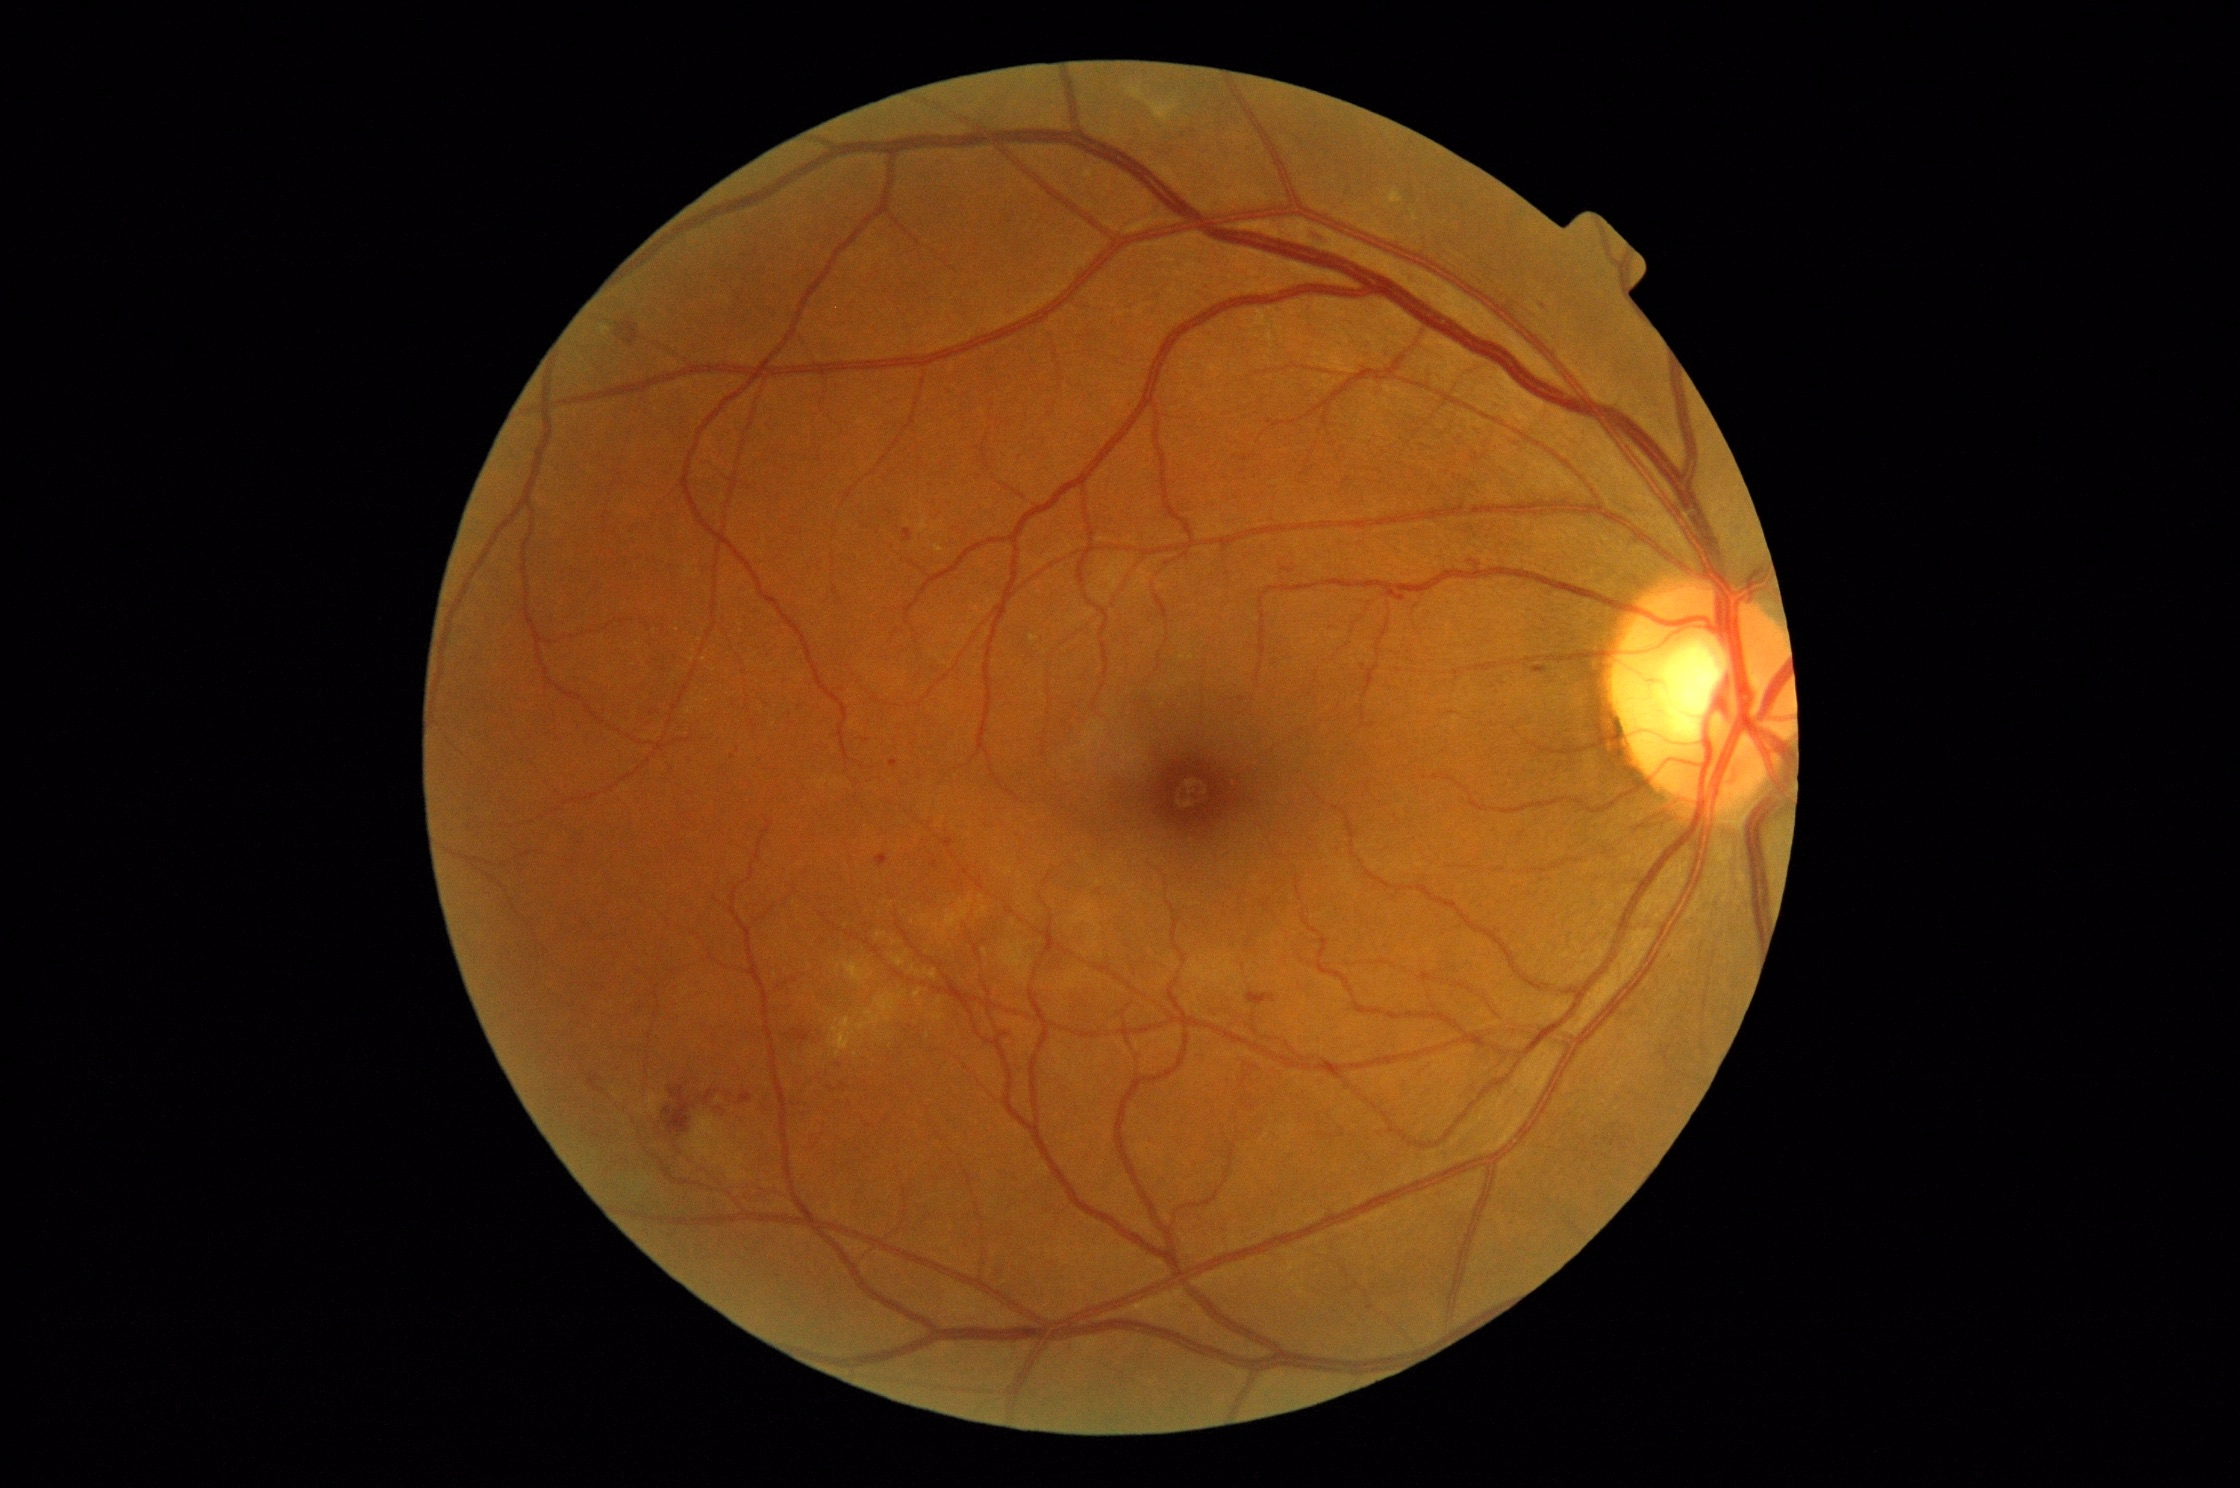
\includegraphics[width=0.8\textwidth]{Figures/DR}
\end{figure}

\begin{figure}[t]
\caption{withoutDR}
\label{fignoDR}
\centering
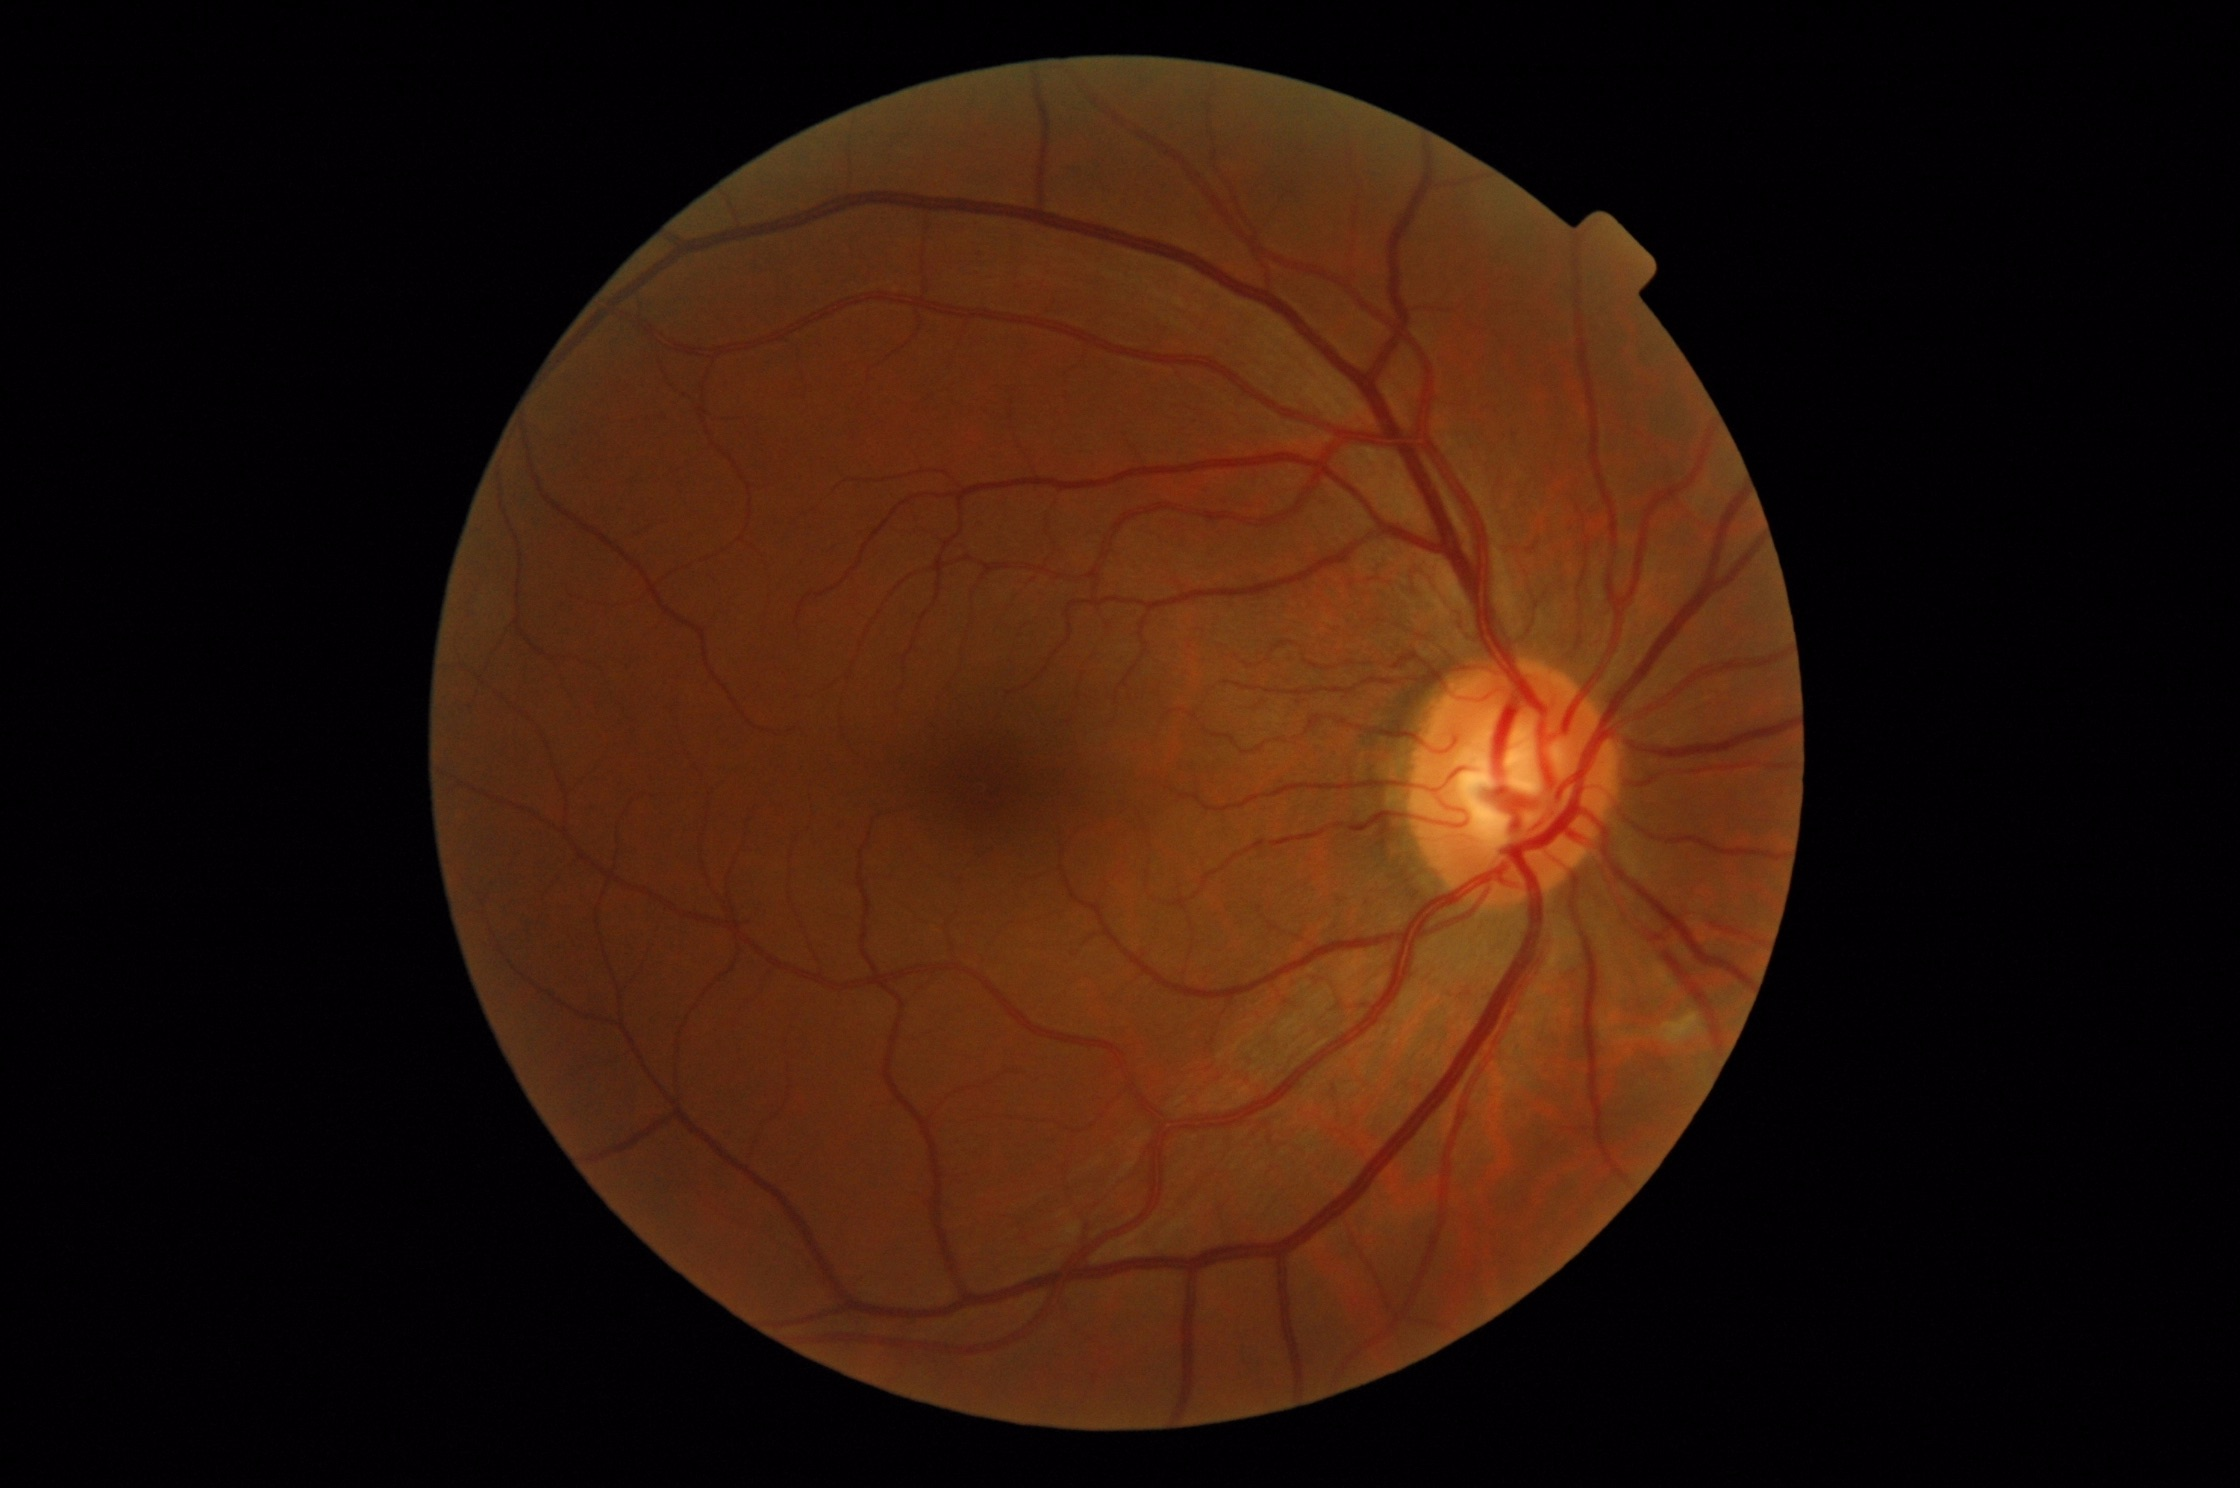
\includegraphics[width=0.8\textwidth]{Figures/NODR}
\end{figure}

\subsection{Neural Networks}
Neural Networks are computational models that are based on the brain architecture to solve different type of problems like image recognition, anomaly detection, signal processing etc. ~\cite{shiffman2012nature} Basically a neural network is an architecture that has a set of input neurons that are activated by inputs (like pixel RGB values for images) and those inputs are weighted and transformed to the other neurons until the architecture arrives the final output neurons. 

\begin{figure}[t]
\caption{Neural Network}
\label{fignn}
\centering
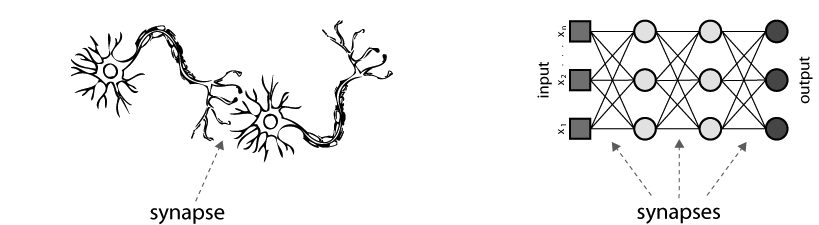
\includegraphics[width=0.8\textwidth]{Figures/nn}
\end{figure}

Figure ~\ref{fignn} shows the similarity between the brain neuron architecture and neural network architecture. 

\subsection{Convolutional Neural Networks}
Convolutional Neural Networks(CNNs) are a type of feed forward neural networks that are based on the animal visual cortex. (http://deeplearning.net/tutorial/lenet.html) CNNs are widely used in different applications of Deep Learning. 
Like regular NNs CNNs also have neurons that have weights and biases that can be learned. The main different between regular NNs and CNNS is that CNNs make the forward function more efficient and creates the neural network architecture with smaller number of parameters learned, which is a lot more efficient. (REF: http://cs231n.github.io/convolutional-networks/) 

\begin{figure}[t]
\caption{Regular Neural Network}
\label{figregnn}
\centering
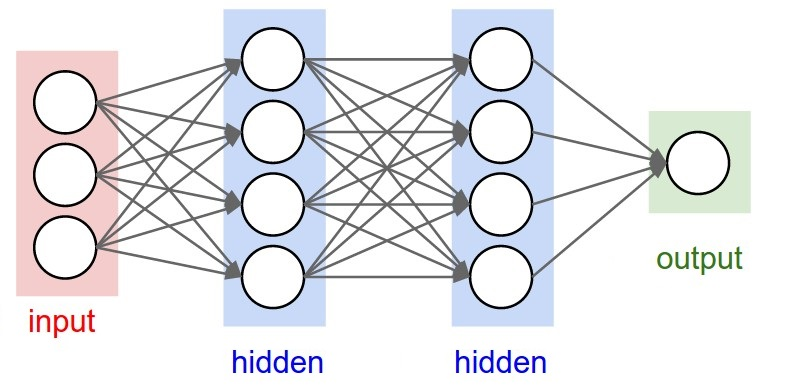
\includegraphics[width=0.8\textwidth]{Figures/regnn}
\end{figure}

In Figure ~\ref{figregnn} a regular neural network architecture can be seen and in Figure ~\ref{figconvnet} shows a sample CNN architecture. 

\begin{figure}[t]
\caption{Convolutional Neural Network}
\label{figconvnet}
\centering
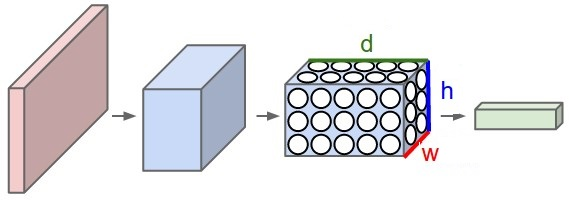
\includegraphics[width=0.8\textwidth]{Figures/convnet}
\end{figure}

CNNs are made of different layers that feedforward the activation of the input neurons to the following layers.The layers are as follows:

\begin{enumerate}
    \item Convolutional Layer
    \item Pooling Layer
    \item Fully Connected Layer
\end{enumerate}

To explain the details of the layers of the CNNs we will use a simple CNN architecture for diabetic retinopathy detection problem. Notice that later we will explain the final CNN architecture we use for the classification problem which will have lots of different layers and parameters etc. For now to explain how CNNs are used for detection of signs of diabetic retinopathy we use the following CNN architecture:\\ 
${INPUT => CONV => RELU => POOL => FC}$. 

\begin{itemize}
    \item INPUT[128x128x3] has the pixel values of the image after preprocessing stage, in our example it is an input image with width 128, height 128 and depth 3.
    \item CONV layer transforms the pixel values of the local regions of the input image by using input neurons' weight and biases. After CONV layer if we use 32 filters, we will have [128x128x32] volume.
    \item RELU layer applies an activation function to the output of CONV layer that does not change the volume [128x128x32]
    \item POOL layer downsamples the width and height dimensions of the volume resulting in [64x64x32].
    \item FC layer classifies the input image to one of the classes (DR and NoDR) resulting in [1x1x2] which has two class scores. Notice that if our problem was to classify input image to 4 classes the output volume would be [1x1x4].
\end{itemize}


\subsection{TensorFlow}
TensorFlow is a machine learning library opensourced by Google for distributed machine learning and deep learning. In this work for convolutional neural networks we use Google's Tensorflow library. (https://www.tensorflow.org) 

\section{Datasets}
\subsection{Messidor Dataset}
The main dataset that we use is called Messidor Dataset ~\cite{decenciere2014feedback} that contains 1200 eye fundus color numerical images. They used a color video 3CCD camera on a Topcon TRC NW6 non-mydriatic retinograph with a 45 degree field of view to capture the images using 8 bits per color plane at 1440*960, 2240*1488 or 2304*1536 pixels. 
They have two medical diagnoses in the dataset: retinopathy grade and risk of macular edema. 

\begin{table}[t]
\centering
\caption{Retinopathy Grade} \label{tab:rg}
\begin{tabular}{|c|c|} \hline
grade & explanation \\ \hline
0 & $(MA = 0) AND (H = 0)$ \\ \hline
1 & $(0 < MA <= 5) AND (H = 0)$\\\hline
2 & $((5 < MA < 15) OR (0 < H < 5)) AND (NV = 0)$ \\\hline
3 & $(MA >= 15) OR (H >=5) OR (NV = 1)$\\\hline
\end{tabular}
\end{table}

Different retinopathy grades are shown in Table ~\ref{tab:rg} where MA: number of microaneurysms, H:number of hemorrhages, NV = 1: neovascularization and NV = 0: no neovascularization. 

\begin{table}[t]
\centering
\caption{Risk of Macular Edema} \label{tab:ma}
\begin{tabular}{|c|c|} \hline
risk & explanation \\ \hline
0 & (No risk): No visible hard exudates \\ \hline
1 & Shortest distance between macula and hard exudates > one papilla diameter\\\hline
2 & Shortest distance between macula and hard exudates <= one papilla diameter \\\hline
\end{tabular}
\end{table}

Different level of macular edema risk are shown in Table ~\ref{tab:ma}.

\section{Preprocessing}
Before training the convolutional neural networks the first thing to do is preprocessing the images. Preprocessing is a must stage since the images in the dataset are produced under different circumstances. For instance not all images have the same resolution and not all of the images are produced under the same lightning. To fix these problems we apply some preprocessing techniques for the images. 

\begin{enumerate}
    \item Blur the images. Blurring the images is a technique in Computer Vision problems that is used for enhancing image structures at different scales.
    \item Cropping the images to bounding box having pixel values above a threshold.
    \item Scaling the images to a certain resolution. In our case we scale all of the images to 128x128.
    \item We apply histogram normalization for each of the RGB channels seperately. Histogram normalization changes the pixel intensity values. This results in areas of lower local contrast gaining a higher contrast by effectively spreading out the most frequent intensity values.
\end{enumerate}

TODO: Rotate the images randomly, both test and train data. 
Aplly contrast, sharpness etc to the images and compare the results. 
Add here an image with different preprocessing steps. 

\section{ConvNET Architecture for Diabetic Retinopathy}
In this section we will explain the convolutional neural network used in this work for diabetic retinopathy detection architecture in detail. 

\begin{table}[t]
\centering
\caption{CNN architecture} \label{tab:cnnarc}
\begin{tabular}{|c|c|c|c|} \hline
layer & input volume & no of filters & nof units \\ \hline
conv & 128x128x3 & 16 & \\ \hline
conv & 128x128x16 & 16 & \\ \hline
pool & 128x128x16 &  & \\ \hline
conv & 64x64x16 & 32 & \\ \hline
conv & 64x64x32 & 32 & \\ \hline
pool & 64x64x32 &  & \\ \hline
conv & 32x32x32 & 64  & \\ \hline
conv & 32x32x64 & 64  & \\ \hline
pool & 32x32x64 &   & \\ \hline
conv & 16x16x64 & 128  & \\ \hline
pool & 16x16x128 &   & \\ \hline
conv & 8x8x128 & 128  & \\ \hline
pool & 8x8x128 &   & \\ \hline
conv & 4x4x128 & 256  & \\ \hline
pool & 4x4x256 &   & \\ \hline
dropout & 2x2x256 & & \\ \hline
fc1 & 2x2x256 & &96 \\ \hline
fc1 & 96x2 & &2 \\ \hline
softmax & & & \\ \hline
\end{tabular}
\end{table}

Table ~\ref{tab:cnnarc} shows the details of the convolutional neural network architecture used for this work. Notice that for the number of units after the second fully connected layer, 2 represents number of output classes, in this case DR and noDR. For the degree of the diabetic retinopathy it would be 4. For all of the convolutional layers stride size is 1 and padding is the same, meaning that the dimension (width, height) does not change. Kernel size for conv layers is always 3x3 in this work. Pool layers use maxpooling with 2x2 pooling window and stride is 2, such that after pooling layer width and height is divided by 2. After all convolutinal layers for the activation rectified linear unit (ReLU) is used. (buraya relu image gelecek ve formul) Similarly after the fully connected layer also ReLU is used. 
We trained the net using adam optimizer (a method for stochastic optimization) ~\cite{kingma2014adam} with  logloss as a loss function. 





